\documentclass[conference]{IEEEtran}
\usepackage[T1]{fontenc}
\usepackage{cite}
\usepackage{amsmath}
\usepackage{graphicx}
\usepackage{booktabs}
\usepackage{url}
\usepackage[hidelinks]{hyperref}
\renewcommand{\topfraction}{0.9}
\renewcommand{\textfraction}{0.1}
\renewcommand{\floatpagefraction}{0.85}

% Algorithm boxes (ruled, numbered lines).
\newcounter{algo}
\newcounter{algline}
\newcommand{\Kw}[1]{\textbf{#1}}
\newcommand{\Ind}{\hspace*{1em}}
\newenvironment{algo}[2]{\begin{figure}[t]\refstepcounter{algo}\label{#2}%
  \hrule height 0.8pt\vspace{2pt}\noindent\textbf{Algorithm \thealgo:} #1\par\vspace{2pt}%
  \hrule height 0.4pt\vspace{2pt}\footnotesize\raggedright
  \begin{list}{\arabic{algline}:}{\usecounter{algline}\setlength{\leftmargin}{1.7em}%
    \setlength{\labelwidth}{1.4em}\setlength{\itemsep}{0pt}\setlength{\parsep}{0pt}\setlength{\topsep}{0pt}}}%
  {\end{list}\vspace{2pt}\hrule height 0.8pt\end{figure}}

\begin{document}

\title{FEVER: Federated Detection and Ingress Blocking\\against Low-Rate Flow Table Overflow in SDN}

\author{\IEEEauthorblockN{Author Name}
\IEEEauthorblockA{Affiliation\\
City, Country\\
email@example.com}}

\maketitle

\begin{abstract}
A low-rate flow table overflow (LOFT) attack fills the flow table of an SDN switch with entries that the
attacker keeps alive by sending one packet to each of them shortly before the idle timeout. New benign
flows then find no room in the table, while the attack traffic stays far below the alarm level of
rate-based detectors. Published defenses train a classifier on the traffic of a single network and fail
when the attacker changes its pattern. In this paper, we propose FEVER, which trains one XGBoost detector
across several SDN controllers without moving their data. The controllers exchange only per-bin gradient
and hessian sums, so that the split search sees the same histograms as XGBoost on the pooled rows. At run
time the detector also drives the mitigation. FEVER evicts the entries it flags and blocks a host at its
ingress port when these evictions or the host's share of the table become outliers. We compare FEVER with six published defenses, reimplemented on
a Mininet, Open vSwitch and Ryu testbed, over seven attacks, two real traffic captures and 532 runs, with
hypotheses fixed before the runs. FEVER harmed 0.011\,\% of benign flows against 1.0\,\% to 5.2\,\% and
kept 84\,\% of new connections working against 21\,\% to 46\,\%; 25 of 33 tests are supported.
Federated training raised the recall on an attack that only another controller had seen from 0.2\,\% to
61\,\%. However, no method stopped a slow attack with spoofed sources, and attackers that stay below
FEVER's volume limit were not blocked.
\end{abstract}

\begin{IEEEkeywords}
software-defined networking, flow table overflow, federated learning, XGBoost, attack mitigation
\end{IEEEkeywords}

\section{Introduction}

Software-defined networking (SDN) separates the control plane from the data plane. An OpenFlow switch
forwards a packet by matching it against the entries of its flow table, and when no entry matches, it
sends the packet to the controller, which decides how the flow is handled and installs a new entry
\cite{mckeown2008openflow}. This design gives the operator fine control over every flow, but it also
ties the forwarding capacity of the switch to the size of its flow table. The table is usually held in
ternary content addressable memory (TCAM), which is fast but expensive and power hungry, so a switch
holds only a few thousand entries. An entry is removed only when it has been idle for longer than its
timeout, or when the controller deletes it.

Cao et~al.\ showed that an attacker can exhaust this table with very little traffic \cite{cao2017loft}.
The attacker opens many flows, each with a different header, and sends one packet to each flow just
before its idle timeout expires. The entries never expire, the table fills, and the switch can no longer
install entries for new benign flows, which are then dropped or wait for an entry to be freed. Because
each attack flow carries only a packet every few seconds, the attack raises neither the packet rate nor
the bandwidth of the link, and detectors that look for traffic volume do not notice it. Tang et~al.\
call the same pattern a slow-rate or low-rate flow table overflow attack \cite{tang2023sftoguard,tang2023ftmaster}.

A series of defenses detect such attacks with a classifier on features of the flow table and of
individual entries, then evict the entries they classify as malicious and, in some cases, block the
source \cite{tang2023sftoguard,tang2023ftmaster,tang2024ftodefender,tang2024ftop,mudgal2024flora,tang2025dmsbtt,jain2025ftshield}.
Each of them is trained and evaluated on the traffic of one network, with the same attack generator at
training and test time, and reports detection rates near 99\,\%. Zeng et~al.\ found that how well
FTMaster detects an attack depends on the eviction policy of the switch, and built an attack that adapts
to it \cite{zeng2024alfo}. A classifier trained on one network therefore learns the attacks that this
network has seen, and may miss an attack whose packet sizes, sources or timing differ.

Moreover, the operators of different networks usually observe different attacks. For example, one
controller may have recorded an attack that imitates benign packet sizes, and another a pulsed attack.
Pooling their recordings would give a better classifier, but flow records reveal the hosts, services and
traffic volumes of each network and are rarely shared between administrative domains. Federated learning
trains a common model without moving the data \cite{mcmahan2017fedavg}, and has been applied to DDoS
detection in multi-controller SDN \cite{fotse2025fedlad,alkhamisi2024fedsec,ali2023lrddos}. These works
average the weights of neural or other models, and none of them addresses flow table overflow.

In this paper, we study whether controllers can train a common detector for LOFT attacks without sharing
their recordings, and whether such a detector helps on a real testbed against attacks that the local
training never saw. We use gradient-boosted trees, the model family used by most published LOFT
defenses, and federate them by exchanging histogram sums instead of model weights. The main
contributions of this paper are as follows:
\begin{itemize}
\item FEVER, a defense that trains an XGBoost detector across controllers by exchanging only gradient and
  hessian histograms, so that every split is chosen as on the pooled data, and that uses the scores of this detector to
  decide which entries to evict and which hosts to block at their ingress port
  (Section~\ref{sec:design}).
\item A comparison with six published defenses reimplemented on a Mininet, Open vSwitch and Ryu testbed
  with two real traffic captures and seven attacks, three of which no controller trained on. The
  hypotheses, measures and tests were fixed before the 532 runs (Sections~\ref{sec:setup}
  and~\ref{sec:results}).
\item An analysis of the cases in which federated training improves the defense, including two attacks
  that FEVER does not stop, and four further studies: benign flash crowds, up to eight colluding
  attackers, the sensitivity to FEVER's settings, and secure aggregation of the exchanged histograms.
\end{itemize}

The rest of the paper is organised as follows. Section~\ref{sec:background} describes flow tables, the
LOFT attack and histogram-based tree training. Section~\ref{sec:related} reviews related work.
Section~\ref{sec:design} presents FEVER, Section~\ref{sec:setup} the testbed and
Section~\ref{sec:results} the results. Section~\ref{sec:discussion} discusses the limitations and
Section~\ref{sec:conclusion} concludes the paper.

\section{Background}
\label{sec:background}

\subsection{Flow tables in OpenFlow switches}

An OpenFlow flow entry consists of match fields, a priority, counters, instructions and timeouts
\cite{mckeown2008openflow}. The counters record the packets and bytes that matched the entry and the
time since it was installed, and the controller reads them with flow statistics requests. A packet that
matches no entry triggers a table miss, and the switch sends it, or its header, to the controller in a
Packet-In message. The controller then installs an entry with a flow modification message, so that the
following packets of the flow are forwarded by the switch alone. An entry with an idle timeout $T$ is
removed when no packet has matched it for $T$ seconds. When the table is full, the switch refuses new
entries and reports a table-full error, or, if configured, evicts an entry by its own policy.

\subsection{The LOFT attack}

The attack of Cao et~al.\ \cite{cao2017loft} has two phases. In the first, the attacker probes the switch
to learn which header fields are matched, the idle timeout and the table capacity, by timing its own
packets: a packet that causes a table miss takes longer, because it passes through the controller. In
the second, it opens flows whose headers differ in a matched field, and refreshes each of them once per
idle timeout. To hold $M$ entries it needs only $M/T$ packets per second. With $M = 1{,}700$ entries,
$T = 10$\,s and 64-byte packets this is 170 packets per second, or about 87\,kbit/s, a rate that does
not stand out among the benign flows of a campus or data-centre network. On hardware switches Cao
et~al.\ overflowed 1,800 TCAM entries at 46\,kbit/s. An attacker can also draw its sources from a pool of
addresses or spoof them, copy the packet sizes of benign traffic, or vary the gap between refreshes,
which makes the attack entries look like benign ones.

\subsection{Histogram-based gradient-boosted trees}

XGBoost \cite{chen2016xgboost} builds an ensemble of regression trees, each fitted to the gradients of
the loss with respect to the current prediction. For a row $i$ with label $y_i$ and prediction $p_i$
under the logistic loss, the first and second derivatives are $g_i = p_i - y_i$ and
$h_i = p_i(1 - p_i)$. The histogram method first divides the range of each feature into at most 256
bins. For a tree node and a feature $j$, it adds up the derivatives of the rows in the node per bin $b$,
\begin{equation}
G_{jb} = \sum_{i \in b} g_i, \qquad H_{jb} = \sum_{i \in b} h_i .
\label{eq:hist}
\end{equation}
A split of the node at a bin boundary sends the rows on the left, with sums $G_L$ and $H_L$, to one child
and the rest, with $G_R$ and $H_R$, to the other. Its gain is
\begin{equation}
\mathcal{G} = \frac{1}{2}\left[\frac{G_L^2}{H_L + \lambda} + \frac{G_R^2}{H_R + \lambda}
 - \frac{(G_L + G_R)^2}{H_L + H_R + \lambda}\right] - \gamma ,
\label{eq:gain}
\end{equation}
where $\lambda$ and $\gamma$ penalise the leaf weights and the number of leaves, and a leaf with sums
$G$ and $H$ receives the weight $w = -G/(H + \lambda)$. The algorithm chooses the split with the largest
gain over all features and bins. Both the gain and the leaf weights depend on the rows only through the
sums in (\ref{eq:hist}), which is what makes the federated training of Section~\ref{sec:design} exact.

\section{Related Work}
\label{sec:related}

\textit{LOFT attacks.} Besides the attack of Cao et~al.\ \cite{cao2017loft}, Tang et~al.\ describe the
same pattern as a slow-rate flow table overflow and study how its rate and the number of entries it
holds affect the switch \cite{tang2023sftoguard}. ALFO adapts the attack to the eviction policy of the
switch, so that the attack entries are not the ones evicted \cite{zeng2024alfo}.

\begin{table}[t]
\centering
\caption{Published LOFT defenses and FEVER.}
\label{tab:related}
\footnotesize
\setlength{\tabcolsep}{2.5pt}
\begin{tabular}{llll}
\toprule
Defense & Detector & Response & Trained on \\
\midrule
FTGuard \cite{zhang2017ftguard} & none (priority) & eviction & -- \\
SFTO-Guard \cite{tang2023sftoguard} & LightGBM & adaptive eviction & one net. \\
FTMaster \cite{tang2023ftmaster} & XGBoost & evict, block source & one net. \\
FTODefender \cite{tang2024ftodefender} & LightGBM-LR & evict, block source & one net. \\
FTOP \cite{tang2024ftop} & random forest & eviction & one net. \\
FloRa \cite{mudgal2024flora} & CatBoost & blacklist, evict & one net. \\
DMS-BTT \cite{tang2025dmsbtt} & CatBoost (two) & eviction & one net. \\
rDefender \cite{kong2024rdefender} & none (port share) & random deletion & -- \\
FTShield \cite{jain2025ftshield} & ensemble in P4 & block host & one net. \\
FEVER & XGBoost & evict, block at ingress & federated \\
\bottomrule
\end{tabular}
\end{table}

\textit{Defenses.} Table~\ref{tab:related} summarises the published defenses. FTGuard evicts entries by
a priority computed from the rate of new flows and the packet count of each flow, without a classifier
\cite{zhang2017ftguard}. SFTO-Guard predicts the number of rules in the table, detects the attack with
LightGBM, and evicts a share of the suspected entries that it adapts to the predicted rule count
\cite{tang2023sftoguard}. FTMaster uses XGBoost both to decide whether the table is under attack and to
classify each entry, then evicts the malicious entries and blocks the source \cite{tang2023ftmaster}.
FTODefender weights four table features by the CRITIC method to detect the attack, and classifies the
entries with a LightGBM and logistic regression model before evicting them and cutting off the source
\cite{tang2024ftodefender}. FTOP predicts the flow count, detects the attack and classifies the entries
with random forests, and also evicts low-scored entries during flash crowds \cite{tang2024ftop}. FloRa
adds new entry features, such as the packet arrival frequency and a spoofed-address indicator, classifies
with CatBoost and blacklists the flagged flows \cite{mudgal2024flora}. DMS-BTT combines a table-state and
a per-entry CatBoost model with two occupancy thresholds: above the first it evicts suspected entries at
once, between the two it runs the detector \cite{tang2025dmsbtt}. rDefender does not use a classifier;
instead, it finds the ports whose share of the table is abnormal and deletes their entries at random
\cite{kong2024rdefender}. FTShield runs an ensemble of classifiers in the P4 pipeline of a Tofino switch
and blocks the attacking host \cite{jain2025ftshield}. All the learning-based defenses train on the
traffic of one network. FEVER keeps the evict-then-block response of FTMaster and FTODefender and changes
how the detector is trained.

\textit{Federated learning for attack detection.} FedAvg \cite{mcmahan2017fedavg} and FedProx
\cite{li2020fedprox} average the weights of models trained locally, and Rahman et~al.\ showed for IoT
intrusion detection that such a federated model approaches a centrally trained one
\cite{rahman2020iotfl}. In SDN, federated models have been trained across controllers to detect DDoS
attacks in large networks \cite{fotse2025fedlad}, attacks in multi-controller networks
\cite{alkhamisi2024fedsec}, low-rate DDoS against the control plane \cite{ali2023lrddos}, and DDoS with a
hybrid convolutional and recurrent network \cite{zhou2025fedddos}. These works exchange model weights and
target attacks that raise the traffic rate or the load on the controller, not the flow table.

\textit{Federated tree models.} Weight averaging does not apply to decision trees. SecureBoost trains
gradient-boosted trees in the vertical setting, where the parties hold different features of the same
rows, and is lossless, that is, it gives the same model as central training \cite{cheng2021secureboost}.
Li et~al.\ train trees in the horizontal setting, where the parties hold different rows, and share
similarity information between parties instead of gradients, at some loss of accuracy
\cite{li2020fedgbdt}. FEVER is horizontal: every controller holds the same features for different flows,
and the controllers add up their gradient histograms, which gives the histograms of (\ref{eq:hist}) on
the pooled rows. Pairwise masking \cite{bonawitz2017secagg} hides each controller's sums from the others.

\section{FEVER}
\label{sec:design}

\subsection{Threat model}

The attacker controls one or more hosts in the network. It knows the idle timeout and the table capacity,
for example from the probing of \cite{cao2017loft}, and it can choose its sending pattern: the number of
new flows per burst, the gap between bursts, the packet sizes, and whether it uses its own address, a
pool of addresses or spoofed sources. One variant (EVX) also knows FEVER's volume limit. Switches and
controllers are trusted. Each controller manages its own network and keeps its traffic recordings
private; the controllers and the aggregator follow the training protocol but may inspect what they
receive.

\subsection{Overview}

\begin{figure*}[t]
\centering
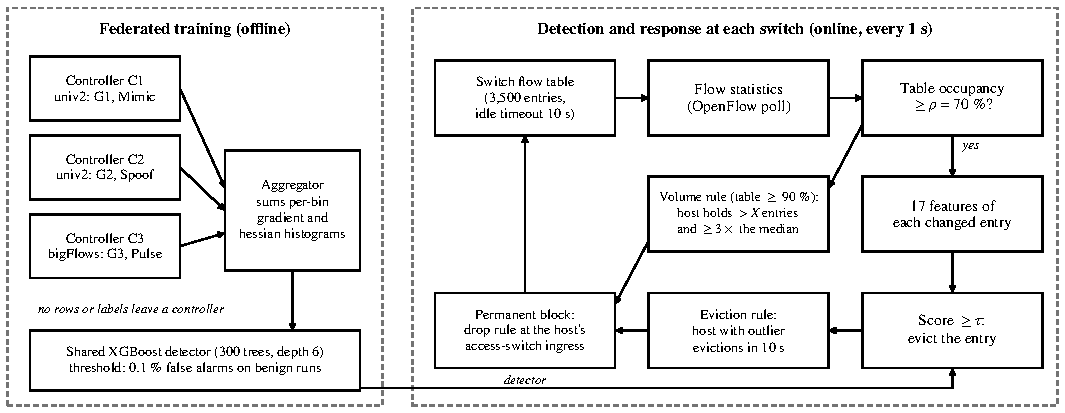
\includegraphics[width=\textwidth]{figs/architecture.pdf}
\caption{Architecture of FEVER.}
\label{fig:arch}
\end{figure*}

Fig.~\ref{fig:arch} shows the architecture of FEVER. It has an offline part, run once by all controllers
together, and an online part, run by each controller for each of its switches. In the offline part,
each controller records labelled flow entries on its own network, computes their features, and takes
part in the federated training of one XGBoost detector through an aggregator. The aggregator sees only
the summed histograms. Each controller then sets its decision threshold on its own benign recordings.
The online part has four modules. The \textit{statistics collector} polls the flow statistics of the
switch every second and keeps, for every entry, the history of its counters and the host that caused
its installation. The \textit{feature extractor} computes the features of each entry whose counters
changed since the previous poll. The \textit{detector} scores these entries with the federated model.
The \textit{mitigator} evicts flagged entries and blocks hosts by the two rules of
Section~\ref{sec:response}. The detector therefore drives the mitigation. Its scores decide which
entries are evicted, and the eviction rule blocks a host on the number of its evicted entries, so only
the volume rule acts without the model. No change to the switches is needed: the controller uses only flow
statistics, flow deletion and flow installation messages of OpenFlow.

\subsection{Features}

For every entry the controller computes 17 features from the flow statistics it polls and from its own
installation log, with no access to packet payloads. Eleven describe the entry: its packet count $n$ and
byte count, its duration $d$, the mean packet size, the packet rate $n/d$, the mean time between packets
$d/n$, the packets since the last poll, the number of polls in which it was idle, the share of polls in
which it was active, and the mean and coefficient of variation of the gaps between its packets. Three
describe the source host of the entry: the number of entries it holds, the number it installed in the
last interval, and the share of them that carry few packets. Three describe the table: its occupancy,
the installation rate and the mean packet interval over all entries. Counts, durations and rates enter
as $\log(1 + x)$, so that the features of a slow attack flow and of a large benign flow lie on a similar
scale. The source features let the detector see that a host keeps many entries with one or two packets
each, which is the signature of the attack even when each entry looks benign by itself.

\subsection{Lossless federated training}

\begin{algo}{Lossless federated training (controller $c$)}{alg:train}
\item[\textbf{In:}] rows $\{(x_i, y_i)\}$ of controller $c$; $K$ trees; depth $D$
\item merge the controllers' quantile sketches into shared bin edges
\item $p_i \gets 0.5$ for all rows $i$
\item \Kw{for} $k = 1, \dots, K$ \Kw{do}
\item \Ind $g_i \gets p_i - y_i$,\; $h_i \gets p_i(1 - p_i)$ for all rows $i$
\item \Ind \Kw{for} each depth $1, \dots, D$ and each open node \Kw{do}
\item \Ind\Ind compute local sums $G^{c}_{jb}, H^{c}_{jb}$ of the node's rows by (\ref{eq:hist})
\item \Ind\Ind send them; receive the totals $G_{jb} = \sum_{c} G^{c}_{jb}$, $H_{jb}$
\item \Ind\Ind choose the split with the largest gain (\ref{eq:gain}) over all $j, b$
\item \Ind\Ind divide the node's own rows between the two children
\item \Ind set each leaf weight $w = -\eta\, G/(H + \lambda)$ from the summed sums
\item \Ind update $p_i$ of the own rows with the new tree
\item[\textbf{Out:}] the same $K$ trees at every controller
\end{algo}

Each controller $c$ holds labelled rows $(x_i, y_i)$ recorded on its own network, with benign traffic and
the attacks it has seen. Algorithm~\ref{alg:train} shows the training. Since the histogram sums are
additive over rows, the sums of a node over all controllers are the sums of the local ones. The
controllers compute them on their own rows and send them to the aggregator, which returns the totals.
Every controller then evaluates the same gains, chooses the same split and computes the same leaf
weights, and each applies the split only to its own rows. No row, feature value or label leaves a
controller. The bin edges come from merging the controllers' quantile sketches, the only step in which
the result can differ from XGBoost on the pooled rows; on our data the two models differ by 0.3 points
of F1. We use $K = 300$ trees of depth $D = 6$, a learning rate $\eta = 0.1$, $\lambda = 1$,
$\gamma = 0$ and 256 bins per feature, and run the exchange through XGBoost's collective communication
library, with the aggregator as its tracker. For one node the messages hold 17 features times 256 bins
times two sums.

The decision threshold $\tau$ is set so that 0.1\,\% of the benign rows of one controller's validation
runs score above it. The threshold is local because it encodes how many false alarms a network accepts.
Section~\ref{sec:secagg} examines a threshold set on the benign scores of all controllers together.

\subsection{Detection and response}
\label{sec:response}

\begin{algo}{Detection and response (one switch, each poll at time $t$)}{alg:loop}
\item[\textbf{In:}] entries $\mathcal{E}$, occupancy $n$, capacity $C$; window $W = 10$\,s
\item \Kw{if} $n < \rho C$ \Kw{then} \Kw{return}
\item $F \gets \{e \in \mathcal{E} :$ counters of $e$ changed and $s(e) \ge \tau\}$
\item delete the entries in $F$; add their counts to $e_h(t)$ per host $h$
\item \Kw{for} each host $h$ seen on the switch \Kw{do}
\item \Ind $E_h \gets \sum_{t - W < t' \le t} e_h(t')$,\; $N_h \gets \sum_{t - W < t' \le t} n_h(t')$
\item $m \gets \max(m_0, \operatorname{median}_h E_h)$,\; $\bar{n} \gets \operatorname{median}_h n_h(t)$
\item \Kw{for} each host $h$ \Kw{do}
\item \Ind \Kw{if} $E_h \ge 50$ \Kw{and} $E_h \ge k m$ \Kw{and} $E_h \ge 0.2 N_h$ \Kw{then} block $h$
\item \Ind \Kw{if} $n \ge 0.9 C$ \Kw{and} $n_h(t) > X$ \Kw{and} $n_h(t) \ge 3 \bar{n}$ \Kw{then} block $h$
\item \Kw{for} each newly blocked host $h$ \Kw{do}
\item \Ind delete its entries; drop its MAC at its ingress port
\end{algo}

Algorithm~\ref{alg:loop} shows the loop that a controller runs on each switch after every poll. It starts
when the occupancy of the table reaches $\rho = 70\,\%$ of its capacity $C$, so that a switch with a
lightly used table costs nothing. FEVER then scores only the entries whose counters changed since the
previous poll, because an unchanged entry has the same features and score as before, and evicts the
entries that score at least $\tau$.

Eviction alone does not stop an attacker who reinstalls its flows, so FEVER also blocks hosts, by two
rules. Let $e_h(t)$ be the evictions of host $h$ at poll $t$, $n_h(t)$ the entries it holds, and $E_h$
and $N_h$ their sums over the last $W = 10$\,s. The \textit{eviction rule} blocks a host whose
evictions are many ($E_h \ge 50$), an outlier among the hosts on the switch ($E_h \ge k m$, with $k = 3$
and the median $m$ floored at $m_0 = 10$), and a substantial part of what it holds
($E_h \ge 0.2 N_h$). The last condition keeps a busy benign host, whose entries are only occasionally
misclassified, from being blocked. The \textit{volume rule} acts when the table is at least 90\,\% full
and does not use the detector. It blocks a host that holds more than $X$ entries and at least three times
as many as the median host. $X$ is set per switch to 1.5 times the largest number of entries that a
benign host held in three benign calibration runs. The volume rule catches attackers whose entries the
detector does not flag, as long as they hold far more of the table than any benign host.

A blocked host loses its entries, and the controller installs a drop rule for its MAC address at the
ingress port of its access switch, so that its packets no longer reach the controller or the other
switches. Blocks are permanent, since a LOFT attacker that is released returns at once.

\section{Experimental Setup}
\label{sec:setup}

\textit{Testbed.} The testbed runs on one machine with Mininet \cite{lantz2010mininet}, Open vSwitch
\cite{pfaff2015ovs} and the Ryu controller \cite{ryu}. The network is a tree of three switches: a core
switch connected to a server and two access switches with three hosts each. Each table holds at most
3,500 entries with an idle timeout of 10\,s, as in \cite{tang2024ftodefender,tang2024ftop,tang2025dmsbtt},
and the controller polls the flow statistics every second. Four benign hosts replay real traffic. Two
attackers, one on each access switch, start at 50\,s. One benign host also opens a new connection to the
server every 0.5\,s, to measure the service that a new benign flow receives. Each run lasts 300\,s.

\textit{Traffic and training data.} T1B is a part of bigFlows \cite{bigflows}, the capture used by
DMS-BTT \cite{tang2025dmsbtt}, replayed at 600 packets/s, and UHt is part 6 of the univ2 data-centre
trace \cite{benson2010imc} at 1,000 packets/s. Three controllers record their own training runs on the
testbed: C1 on univ2 with the attacks G1 and Mimic, C2 on univ2 with G2 and Spoof, and C3 on bigFlows
with G3 and Pulse. No controller trained on the part of univ2 used in UHt, and the training, validation
and test runs use different seeds.

\textit{Attacks.} Every attack follows the pattern used by DMS-BTT \cite{tang2025dmsbtt}. In each burst
the attacker re-sends a packet on each of its live flows and opens $S$ new flows until it holds $M$
flows. Bursts are sent at 1,500 packets/s with a random gap $t_1$ between them (Table~\ref{tab:attacks}).
Mimic and Aware draw their sources from a pool of 256 addresses and copy the packet sizes of the benign
traffic; Aware refreshes every 2 to 3\,s. Slow opens only 45 flows per burst from spoofed sources. EVX
holds 628 flows per attacker, below FEVER's volume limit. Aware, Slow and EVX were seen by no controller
in training; G1 and G3 appear only in the training data.

\begin{table}[t]
\centering
\caption{Attack parameters (per attacker).}
\label{tab:attacks}
\footnotesize
\setlength{\tabcolsep}{3pt}
\begin{tabular}{llrlrll}
\toprule
Attack & Sources & $S$ & $t_1$ (s) & $M$ & Packets & Trained by \\
\midrule
G2 & own & 100 & 5.5--9.0 & 1{,}700 & 64 B & C2 \\
Spoof & spoofed & 100 & 5.5--9.0 & 1{,}700 & 64 B & C2 \\
Pulse & own & 300 & 5.0--8.0 & 1{,}700 & 64 B & C3 \\
Mimic & pool of 256 & 100 & 6.0--9.5 & 1{,}700 & benign & C1 \\
Aware & pool of 256 & 100 & 2.0--3.0 & 1{,}700 & benign & none \\
Slow & spoofed & 45 & 8.0--9.8 & 1{,}700 & benign & none \\
EVX & own & 100 & 5.5--9.0 & 628 & 64 B & none \\
\bottomrule
\end{tabular}
\end{table}


\textit{Compared methods.} We compare FEVER with no defense and with six published defenses that we
reimplemented from their papers: FTMaster, FTOP, FTODefender, FloRa, DMS-BTT and rDefender. Their
classifiers are trained on C3's recordings, as each paper trains on one network, and, to compare at equal
data, also on the pooled recordings of C1 to C3. Four ablations of FEVER remove, in turn, the federated
training (detector trained on C3 only), the volume rule, the detector, and ingress blocking.

\textit{Measures and tests.} \textit{Benign harm} is the share of benign flows that were refused at least
once, never installed, dropped by a rule, or whose first packet was lost. \textit{Attack occupancy} is
the share of the table held by attack entries after the attack starts, averaged over the polls and the
three switches. \textit{New-connection success} is the share of probe connections that succeed after the
attack starts. Each combination of trace, attack and method runs with three seeds (G2, Spoof, Pulse and
all UHt cells) or five (Mimic, Aware, Slow and EVX). Six hypotheses were fixed before the runs. H1--H3
state that FEVER harms fewer benign flows, leaves a lower attack occupancy and keeps new-connection
success no more than 5 points below each baseline on G2, Spoof, Pulse, Mimic and Aware (19 seed-paired
runs per baseline). H4 compares FEVER with the baselines trained on pooled data, H5 tests the occupancy
on Slow, EVX and UHt, and H6 compares FEVER with its own detector trained on C3 only. Each of the 33 tests
is a one-sided exact sign test with Holm's correction \cite{holm1979} at $\alpha = 0.05$.

\section{Results}
\label{sec:results}

\begin{table*}[t]
\centering
\caption{Comparative experiment results.}
\label{tab:main}
\footnotesize
\setlength{\tabcolsep}{3pt}
\begin{tabular}{llrrrrrrrr}
\toprule
Trace & Attack & No defense & FTMaster & FTOP & FTODefender & FloRa & DMS-BTT & rDefender & FEVER \\
\midrule
\multicolumn{10}{l}{\textit{Benign flows harmed (\%)}} \\
\midrule
T1B & G2 & 10.60 & 0.02 & 2.11 & 0.26 & 0.20 & 0.60 & 4.02 & 0.00 \\
 & Mimic & 5.60 & 2.34 & 4.63 & 2.80 & 4.15 & 1.54 & 3.04 & 0.02 \\
 & Spoof & 12.64 & 0.90 & 0.70 & 1.02 & 2.40 & 0.10 & 4.03 & 0.00 \\
 & Slow & 0.00 & 0.04 & 0.86 & 0.31 & 0.15 & 0.09 & 0.00 & 0.01 \\
 & Pulse & 3.89 & 0.03 & 2.02 & 0.23 & 3.18 & 0.02 & 1.64 & 0.01 \\
 & Aware & 12.91 & 7.88 & 1.73 & 9.09 & 12.08 & 1.87 & 2.27 & 0.01 \\
 & EVX & 0.00 & 0.01 & 0.00 & 0.25 & 0.09 & 0.02 & 0.00 & 0.01 \\
UHt & G2 & 38.86 & 0.00 & -- & -- & -- & 0.00 & 14.87 & 0.00 \\
 & Mimic & 29.60 & 25.19 & -- & -- & -- & 9.24 & 10.80 & 0.10 \\
 & Aware & 57.15 & 46.30 & -- & -- & -- & 9.22 & 9.96 & 0.01 \\
\midrule
\multicolumn{10}{l}{\textit{Attack occupancy (\%)}} \\
\midrule
T1B & G2 & 39.5 & 24.9 & 30.8 & 0.3 & 14.0 & 26.8 & 34.1 & 4.8 \\
 & Mimic & 37.7 & 36.4 & 32.7 & 36.1 & 36.9 & 33.3 & 34.1 & 4.9 \\
 & Spoof & 39.7 & 28.6 & 29.9 & 11.2 & 21.4 & 25.9 & 33.8 & 4.6 \\
 & Slow & 21.2 & 20.8 & 21.0 & 20.5 & 20.8 & 20.3 & 21.1 & 19.7 \\
 & Pulse & 30.3 & 18.4 & 24.1 & 0.2 & 29.7 & 20.1 & 28.7 & 1.9 \\
 & Aware & 49.9 & 48.3 & 44.3 & 48.8 & 49.0 & 43.8 & 42.8 & 14.1 \\
 & EVX & 20.6 & 20.5 & 20.6 & 0.2 & 14.3 & 14.1 & 20.6 & 17.7 \\
UHt & G2 & 44.5 & 27.1 & -- & -- & -- & 30.7 & 37.5 & 7.7 \\
 & Mimic & 42.1 & 41.4 & -- & -- & -- & 36.7 & 36.8 & 8.4 \\
 & Aware & 53.9 & 53.3 & -- & -- & -- & 43.4 & 43.2 & 7.0 \\
\midrule
\multicolumn{10}{l}{\textit{New-connection success (\%)}} \\
\midrule
T1B & G2 & 31.1 & 41.2 & 31.3 & 100.0 & 70.0 & 28.6 & 31.4 & 98.8 \\
 & Mimic & 32.3 & 31.6 & 32.3 & 29.1 & 30.7 & 27.8 & 32.9 & 98.0 \\
 & Spoof & 31.5 & 29.2 & 31.7 & 20.5 & 20.4 & 28.8 & 31.2 & 97.0 \\
 & Slow & 70.6 & 69.0 & 71.3 & 61.2 & 68.3 & 61.9 & 70.0 & 74.3 \\
 & Pulse & 12.7 & 61.6 & 11.6 & 100.0 & 12.0 & 11.2 & 12.1 & 96.9 \\
 & Aware & 12.8 & 12.1 & 12.8 & 12.0 & 12.4 & 10.9 & 12.5 & 46.4 \\
 & EVX & 96.5 & 88.1 & 81.8 & 100.0 & 93.3 & 95.1 & 99.7 & 98.6 \\
UHt & G2 & 60.4 & 98.3 & -- & -- & -- & 75.1 & 51.8 & 99.9 \\
 & Mimic & 61.0 & 53.4 & -- & -- & -- & 48.9 & 55.9 & 99.7 \\
 & Aware & 20.2 & 19.0 & -- & -- & -- & 17.9 & 19.3 & 89.8 \\
\bottomrule
\end{tabular}
\end{table*}

\begin{table}[t]
\centering
\caption{Outcome of the hypothesis tests (wins of FEVER / pairs).}
\label{tab:tests}
\footnotesize
\setlength{\tabcolsep}{2.6pt}
\begin{tabular}{lrrrrrr}
\toprule
 & FTMaster & FTOP & FTOD. & FloRa & DMS-BTT & rDef. \\
\midrule
H1 Harm & 17/19$^\dagger$ & 19/19$^\dagger$ & 19/19$^\dagger$ & 19/19$^\dagger$ & 16/19$^\dagger$ & 19/19$^\dagger$ \\
H2 Occupancy & 19/19$^\dagger$ & 19/19$^\dagger$ & 13/19 & 19/19$^\dagger$ & 19/19$^\dagger$ & 19/19$^\dagger$ \\
H3 New conn. & 19/19$^\dagger$ & 19/19$^\dagger$ & 18/19$^\dagger$ & 19/19$^\dagger$ & 19/19$^\dagger$ & 19/19$^\dagger$ \\
H4 Pooled & 10/10$^\dagger$ & 10/10$^\dagger$ & 10/10$^\dagger$ & 10/10$^\dagger$ & 10/10$^\dagger$ & -- \\
H5 Slow, EVX & 5/10 & 8/10 & 2/10 & 4/10 & 3/10 & 9/10 \\
H5 UHt & 9/9$^\dagger$ & -- & -- & -- & 9/9$^\dagger$ & 9/9$^\dagger$ \\
\bottomrule
\multicolumn{7}{l}{$^\dagger$ supported (sign test, Holm-corrected over 33 tests, $\alpha = 0.05$).}
\end{tabular}
\end{table}

\begin{figure*}[t]
\centering
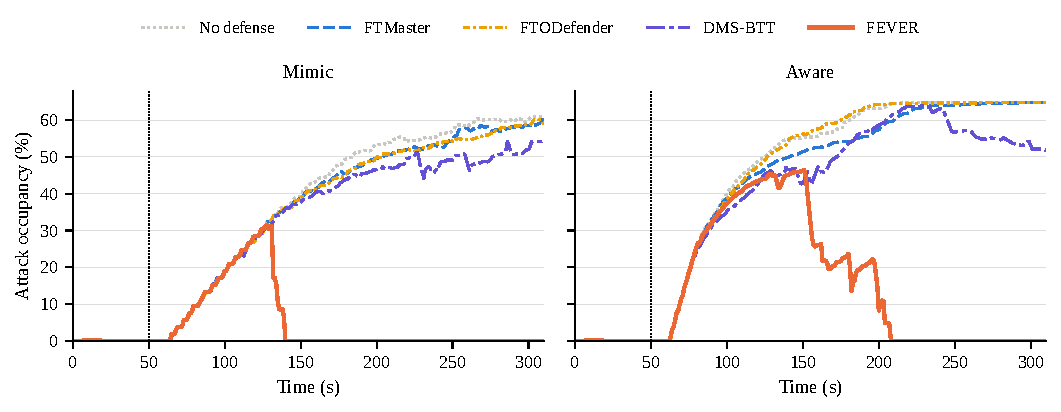
\includegraphics[width=\textwidth]{figs/fig_timeline.pdf}
\caption{Attack occupancy over time on T1B (median over five seeds). The dotted line marks the start of the attack.}
\label{fig:timeline}
\end{figure*}
\begin{figure*}[t]
\centering
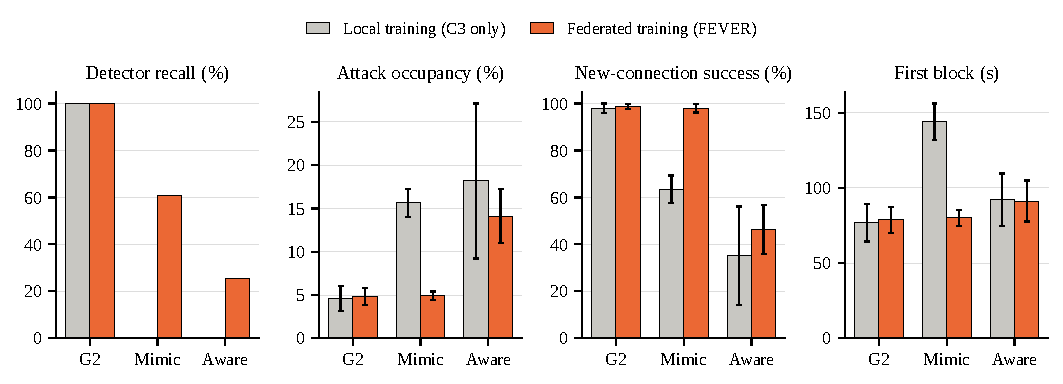
\includegraphics[width=\textwidth]{figs/fig_fl_effect.pdf}
\caption{Effect of federated training on T1B (mean and s.d. over seeds).}
\label{fig:fleffect}
\end{figure*}
\begin{table*}[t]
\centering
\caption{Ablation study.}
\label{tab:ablation}
\footnotesize
\begin{tabular}{llrrrrr}
\toprule
Attack & Variant & Harm (\%) & Occupancy (\%) & New-connection success (\%) & Lost first packets (\%) & First block (s) \\
\midrule
G2 & FEVER & 0.003 (0.006) & 4.82 (0.95) & 98.8 (1.1) & 0.15 (0.16) & 79 (9) \\
 & w/o sharing & 0.017 (0.015) & 4.61 (1.44) & 98.0 (2.0) & 0.15 (0.18) & 77 (13) \\
 & w/o volume rule & 0.003 (0.006) & 4.80 (1.05) & 98.1 (2.0) & 0.12 (0.09) & 78 (10) \\
 & w/o detector & 0.000 (0.000) & 10.88 (1.36) & 79.9 (2.1) & 1.12 (1.47) & 116 (6) \\
 & w/o ingress blocking & 0.003 (0.006) & 24.79 (0.16) & 84.1 (23.0) & 1.50 (1.60) & 77 (11) \\
\midrule
Mimic & FEVER & 0.020 (0.016) & 4.90 (0.51) & 98.0 (1.9) & 0.03 (0.04) & 80 (5) \\
 & w/o sharing & 3.090 (5.214) & 15.67 (1.62) & 63.4 (5.9) & 4.77 (1.71) & 144 (12) \\
 & w/o volume rule & 0.012 (0.008) & 4.79 (0.74) & 98.3 (2.0) & 0.03 (0.05) & 80 (6) \\
 & w/o detector & 0.000 (0.000) & 14.12 (1.53) & 67.7 (4.9) & 2.63 (1.11) & 135 (8) \\
 & w/o ingress blocking & 0.012 (0.022) & 22.90 (2.43) & 62.0 (23.7) & 1.43 (1.63) & 79 (7) \\
\midrule
Aware & FEVER & 0.010 (0.017) & 14.12 (3.12) & 46.4 (10.4) & 15.68 (5.43) & 91 (14) \\
 & w/o sharing & 2.744 (4.212) & 18.18 (8.96) & 35.2 (21.0) & 25.36 (17.91) & 92 (17), 4 of 5 \\
 & w/o volume rule & 1.452 (1.778) & 42.64 (5.08) & 11.3 (2.1) & 50.31 (3.94) & 205 (33), 4 of 5 \\
 & w/o detector & 0.000 (0.000) & 10.40 (2.29) & 55.4 (15.0) & 9.76 (5.83) & 76 (10) \\
 & w/o ingress blocking & 0.020 (0.028) & 34.70 (1.91) & 11.2 (2.0) & 34.47 (8.68) & 97 (13) \\
\bottomrule
\end{tabular}
\end{table*}


\subsection{Comparison with published defenses}

Table~\ref{tab:main} gives the results per attack and Table~\ref{tab:tests} the tests; 25 of the 33 are
supported. Over the 19 seed-paired runs of G2, Spoof, Pulse, Mimic and Aware on T1B, FEVER harmed
0.011\,\% of benign flows, against 1.0\,\% to 5.2\,\% for the baselines, and harmed none in the runs
without an attack. It kept 84.2\,\% of new connections working, and 97\,\% to 99\,\% under G2, Spoof,
Pulse and Mimic, where most baselines fell to between 11\,\% and 41\,\%. The attackers held 6.8\,\% of
the table under FEVER and 24.2\,\% to 35.5\,\% under the baselines. The largest differences occur under
Mimic and Aware: FEVER held them to 4.9\,\% and 14.1\,\% of the table, against 33\,\% to 49\,\%, and also
held a lower occupancy than every baseline trained on the pooled data (H4). On UHt, a capture no
controller trained on, FEVER held the attackers to 7.7\,\% against 37.0\,\% to 40.6\,\% for FTMaster,
DMS-BTT and rDefender. Fig.~\ref{fig:timeline} shows why: the baselines keep evicting attack entries, but
the attackers reinstall them, while under FEVER the attack entries are gone by about 140\,s under Mimic
and 210\,s under Aware, once the attackers are blocked.

However, FEVER did not outperform every baseline on every attack. FTODefender held G2, Pulse and EVX at
about 0.2\,\%, below FEVER, so H2 fails against it; the price was a benign harm of 3.4\,\% and a
new-connection success of 45.6\,\%. Under Slow, every method left about 20\,\% of the table to the
attackers, and FEVER's volume rule let the EVX attackers keep 17.7\,\%, so H5 is not supported on T1B.

\subsection{Effect of federated training}

Federated training improves detection mainly on the attacks that the local controller has not seen
(Fig.~\ref{fig:fleffect}). Offline, it raised the recall on attacks seen only by another controller from
75.8\,\% to 90.5\,\%, and on Mimic from 0.2\,\% to 60.9\,\%. On the testbed, FEVER with the federated
detector blocked the Mimic attackers 64\,s earlier than with C3's detector, lowered the occupancy from
15.7\,\% to 4.9\,\% and raised new-connection success from 63\,\% to 98\,\%. Under Aware the gain was
smaller (14.1\,\% against 18.2\,\%), so over Mimic and Aware together H6 is not supported (8 of 10 pairs,
$p = 0.38$ after correction). FedAvg and FedProx on a small neural network, and federated bagging of
XGBoost trees, gained nothing over local training on these attacks, while the lossless scheme needed
2.6\,GB of exchanged histograms and 38\,s of training (Table~\ref{tab:fedcost} in the appendix).

\subsection{Ablation and overhead}

Table~\ref{tab:ablation} removes one part of FEVER at a time. Without ingress blocking the occupancy rose
to 23\,\% to 35\,\% under all three attacks, the largest single effect. Without the volume rule it rose
from 14.1\,\% to 42.6\,\% under Aware. Without the detector only the volume rule blocks. The first block then came
37\,s to 55\,s later under G2 and Mimic and the occupancy more than doubled, from 4.8\,\% to 10.9\,\%
and from 4.9\,\% to 14.1\,\%. Under Aware the detector did not help, as the volume rule alone
blocked earlier (76\,s against 91\,s). Without federated training the occupancy under Mimic rose from
4.9\,\% to 15.7\,\% and the first block came 64\,s later, so the mitigation depends on what the
federated model learned and not only on having a detector. FEVER took 20.8\,ms per decision, close to no defense (19.4\,ms) and
below every baseline, used the least controller CPU (62\,\%) and the most memory (253\,MB), for its
300-tree model (Table~\ref{tab:overhead}).

\subsection{Flash crowds, more attackers and settings}

We added three 12\,s bursts of new benign flows to the T1B replay, with no attacker, in tables of 2,000
entries so that the bursts filled the core table. With the crowd spread over the four benign hosts, no
method blocked a benign host and FEVER harmed 0.02\,\% of benign flows. With the whole crowd sent by one
host, FEVER blocked that host in 11 of 13 runs (95\,\% interval 55\,\% to 98\,\%), and since most blocks
came in the first crowd, its harm reached 20.8\,\% against 0.06\,\% without a defense in the ten runs of
a second preregistered study. No other method blocked a host. With four and eight attackers, FEVER
blocked every G2 attacker and kept a lower occupancy than FTMaster and DMS-BTT in all paired runs; under
EVX, four or more attackers push the table past $\rho$, and the eviction rule blocked 32 of 36. With
eight attackers its harm was 0.9\,\% under G2 and 2.0\,\% under EVX, against 16.3\,\% and 12.1\,\%
without a defense. Changing $\rho$, $k$ or the factor of $X$ one at a time (90 runs,
Table~\ref{tab:sens}) kept harm and occupancy within 0.5 and 5 points of FEVER's in 17 of 18 cases; the
exception is $\rho = 0.8$ under Mimic (15.0\,\% occupancy). No setting blocked a benign host without an
attack, and every setting blocked the single crowd host.

\subsection{Detection accuracy}

Offline, on the T1B test recordings, the classifiers trained on C3 alone reach an F1 of 78.5\,\% over
all attacks, because they miss Mimic, Slow and Aware, while FEVER's federated detector reaches 86.8\,\%;
on the attacks C3 saw, all reach about 99.8\,\% (Table~\ref{tab:detect}). FEVER's false alarms on T1B,
0.79\,\%, exceed the 0.1\,\% its threshold was set for, because the threshold was calibrated on another
capture. Nevertheless, FEVER did not block any benign host in these runs.

\subsection{Secure aggregation and a federated threshold}
\label{sec:secagg}

The histogram sums that a controller sends describe its traffic. We added the pairwise additive masks of
Bonawitz et~al.\ \cite{bonawitz2017secagg}: each pair of controllers agrees on a key by X25519
\cite{rfc7748}, and each controller adds a ChaCha20 \cite{rfc8439} keystream per pair to its sums, with
opposite signs within a pair, so that the aggregator learns only the total. The sums are encoded in fixed
point modulo $2^{64}$, so the masks cancel exactly. Masked and unmasked training gave the same model bit
for bit, at 2.1\,\% more training time. The same masked sum lets the controllers set $\tau$ on their
pooled benign scores without revealing them, which lowered FEVER's false alarms on T1B from 0.79\,\% to
0.69\,\%, still above the 0.1\,\% target.

\section{Discussion and Limitations}
\label{sec:discussion}

The results indicate that ingress blocking and the detector play different roles. Ingress blocking keeps
the table free; without it, FEVER left the attackers 23\,\% to 35\,\% of the table, because evicted
entries were installed again within seconds. The detector determines how early the block comes, and its
quality depends on whether some controller has seen a similar attack. Federated training therefore
improved the results under Mimic, but added little under G2, which the local detector already
recognises, and under Aware, which no controller had seen.

The testbed is small, with one machine, three switches, at most eight attackers and runs of 300\,s. The
baselines are reimplementations, and some details, such as FTODefender's blocking rule and DMS-BTT's
thresholds, follow our reading of their papers. A crowd sent by a single host looks to FEVER like an
attacker, and a per-host rule cannot tell them apart by volume alone. Finally, no method defends against
Slow, whose spoofed sources spread its entries over many addresses, and EVX shows that two attackers who
know the volume limit can evade it; with four or more, the eviction rule blocked most of them.

\section{Conclusion}
\label{sec:conclusion}

FEVER trains a flow-entry detector across SDN controllers without moving their recordings, and uses its
scores to drive eviction and ingress blocking. On a testbed with real traffic, seven attacks and six reimplemented
defenses, it harmed fewer benign flows and kept more new connections working than every baseline, and
federated training let a controller detect an attack it had never recorded. Detecting slow attacks with
spoofed sources, telling a flash crowd from one host apart from an attack, and setting a threshold that
transfers to a new network are left for future work.

\bibliographystyle{IEEEtran}
\bibliography{refs}

\appendices

\section{Further results}

Table~\ref{tab:fedcost} compares federated training schemes on the same data, Table~\ref{tab:detect}
scores each classifier offline on the T1B test recordings, Table~\ref{tab:overhead} gives the
controller's cost over all T1B runs, and Table~\ref{tab:sens} the study of FEVER's settings.

\begin{table*}[t]
\centering
\caption{Federation cost of the detector.}
\label{tab:fedcost}
\footnotesize\setlength{\tabcolsep}{4pt}
\begin{tabular}{llrrrrrr}
\toprule
Training & Shared & Rounds & Data (MB) & Time (s) & F1 (\%) & Rec., other ctrl. (\%) & Rec., Mimic (\%) \\
\midrule
Local only & nothing & -- & 0 & -- & 78.4 & 75.8 & 0.2 \\
FedAvg & weights & 30 & 0.4 & 32 & 74.7 & 70.7 & 0.1 \\
FedProx & weights & 30 & 0.4 & 27 & 75.9 & 71.4 & 1.1 \\
Federated XGBoost bagging & trees & 100 & 173 & 212 & 78.5 & 75.8 & 0.1 \\
Lossless federated XGBoost (FEVER) & histograms & 300 & 2{,}601 & 38 & 86.8 & 90.5 & 60.9 \\
Lossless, secure aggregation & masked histograms & 300 & 6{,}331 & 796 & 86.8 & 90.4 & 60.4 \\
Pooled XGBoost & rows and labels & 1 & 27.6 & -- & 86.5 & 90.5 & 61.1 \\
\bottomrule
\end{tabular}
\end{table*}

\begin{table*}[t]
\centering
\caption{Detection performance on T1B.}
\label{tab:detect}
\footnotesize
\begin{tabular}{llllrrrrr}
\toprule
Method & Training & Threshold & Test attacks & Accuracy (\%) & Precision (\%) & Recall (\%) & F1 (\%) & False alarms (\%) \\
\midrule
FTMaster & C3 only & 0.5 (paper) & All & 75.32 & 99.80 & 64.66 & 78.48 & 0.33 \\
FTOP & C3 only & 0.5 (paper) & All & 75.35 & 99.84 & 64.67 & 78.49 & 0.32 \\
FloRa & C3 only & 0.5 (paper) & All & 75.34 & 99.82 & 64.68 & 78.50 & 0.32 \\
DMS-BTT & C3 only & 0.5 (paper) & All & 75.35 & 99.82 & 64.68 & 78.50 & 0.32 \\
\midrule
FTMaster & C1--C3 pooled & 0.5 (paper) & All & 89.40 & 98.36 & 86.20 & 91.88 & 3.09 \\
FTOP & C1--C3 pooled & 0.5 (paper) & All & 88.89 & 98.16 & 85.63 & 91.47 & 3.65 \\
FloRa & C1--C3 pooled & 0.5 (paper) & All & 87.50 & 98.75 & 83.09 & 90.25 & 2.58 \\
DMS-BTT & C1--C3 pooled & 0.5 (paper) & All & 87.85 & 98.31 & 83.98 & 90.58 & 3.25 \\
\midrule
FTMaster & C1--C3 pooled & 0.1\% benign & All & 80.95 & 99.83 & 72.74 & 84.16 & 0.22 \\
FTOP & C1--C3 pooled & 0.1\% benign & All & -- & -- & -- & -- & -- \\
FloRa & C1--C3 pooled & 0.1\% benign & All & 79.26 & 99.87 & 70.28 & 82.51 & 0.20 \\
DMS-BTT & C1--C3 pooled & 0.1\% benign & All & 78.10 & 99.81 & 68.65 & 81.35 & 0.30 \\
\midrule
FEVER & C1--C3 federated & 0.1\% benign & All & 83.73 & 99.74 & 76.82 & 86.79 & 0.79 \\
\midrule
FTMaster & C3 only & 0.5 (paper) & G3, Pulse & 99.81 & 99.82 & 99.86 & 99.84 & 0.33 \\
FTOP & C3 only & 0.5 (paper) & G3, Pulse & 99.82 & 99.85 & 99.85 & 99.85 & 0.32 \\
FloRa & C3 only & 0.5 (paper) & G3, Pulse & 99.82 & 99.84 & 99.87 & 99.85 & 0.32 \\
DMS-BTT & C3 only & 0.5 (paper) & G3, Pulse & 99.82 & 99.84 & 99.87 & 99.85 & 0.32 \\
FEVER & C1--C3 federated & 0.1\% benign & G3, Pulse & 99.77 & 99.70 & 99.91 & 99.81 & 0.79 \\
\bottomrule
\end{tabular}
\end{table*}

\begingroup\renewcommand{\small}{\footnotesize}\begin{table}[t]
\centering
\caption{Controller overhead.}
\label{tab:overhead}
\footnotesize
\setlength{\tabcolsep}{2pt}
\begin{tabular}{lrrrr}
\toprule
Method & Decision (ms) & CPU (\%) & Memory (MB) & Packet-In ($10^3$) \\
\midrule
No defense & 19.4 (5.4) & 76.5 (12.1) & 199 (30) & 99.8 (16.5) \\
FTMaster & 53.7 (46.3) & 78.3 (11.7) & 205 (33) & 96.0 (17.3) \\
FTOP & 103.3 (81.4) & 77.8 (12.3) & 233 (41) & 98.4 (16.8) \\
FTODefender & 55.8 (46.7) & 70.0 (16.6) & 191 (34) & 84.0 (13.5) \\
FloRa & 35.2 (17.4) & 75.3 (13.3) & 200 (37) & 94.7 (15.4) \\
DMS-BTT & 58.3 (41.8) & 77.8 (11.5) & 232 (52) & 108.3 (28.6) \\
rDefender & 50.1 (38.9) & 77.1 (11.7) & 214 (50) & 103.1 (18.8) \\
FEVER & 20.8 (15.5) & 62.2 (10.6) & 253 (19) & 87.7 (13.7) \\
\bottomrule
\end{tabular}
\end{table}
\endgroup
\begin{table}[t]
\centering
\caption{Sensitivity of FEVER to its settings on T1B.}
\label{tab:sens}
\footnotesize
\setlength{\tabcolsep}{3pt}
\begin{tabular}{lrrrrr}
\toprule
& \multicolumn{3}{c}{Attack occupancy (\%)} & Benign blocks, & Crowd host \\
\cmidrule(lr){2-4}\cmidrule(lr){5-5}\cmidrule(lr){6-6}
Setting & G2 & Mimic & Aware & no attack & blocked \\
\midrule
FEVER & 4.8 & 4.9 & 14.3 & 0 & 2 of 3 \\
$\rho = 0.6$ & 2.2 & 2.2 & 15.8 & 0 & 3 of 3 \\
$\rho = 0.8$ & 6.2 & 15.0 & 12.0 & 0 & 3 of 3 \\
$k = 2$ & 4.6 & 4.9 & 12.7 & 0 & 3 of 3 \\
$k = 4$ & 4.6 & 4.9 & 11.7 & 0 & 3 of 3 \\
$X$ at 1.25 times & 4.6 & 4.7 & 12.3 & 0 & 3 of 3 \\
$X$ at 2.0 times & 4.6 & 4.7 & 13.1 & 0 & 3 of 3 \\
\bottomrule
\end{tabular}
\end{table}


\end{document}
